\documentclass{beamer}
\usepackage{graphicx}
\usepackage{caption}
\usepackage{subcaption}
\setbeamertemplate{caption}[numbered]
\captionsetup{font=tiny}
\usepackage{tikz}
\usepackage{pgfplots}
\usepackage{multicol}
\usepackage{amsmath}
\usepackage{dsfont}
\usepackage{booktabs}
\usepackage{array}
\usepackage{multirow}
\usetikzlibrary{trees, positioning}
\usetheme{Frankfurt}
\pgfplotsset{compat=1.18}
\usepackage{helvet} \renewcommand{\familydefault}{\sfdefault}
\setbeamertemplate{headline}{\leavevmode\hbox{}}
\graphicspath{{./}{../comparison_unsupervised_object_discovery/VOC07/}{../ppt_results/object_detection/}}

\title{TokenCut: Extensions for Unsupervised Object Discovery}
\author{Bitupan Arandhara, Dwaipayan Haldar \protect\linebreak Indian Institute of Science}
\date{\today}

\begin{document}

% ---------- TITLE ----------
\begin{frame}
\maketitle
\end{frame}

% ---------- FRAME 1 ----------
\begin{frame}{TokenCut: Step 1 — Graph Construction}
\begin{itemize}
    \item A fully connected undirected graph $\mathcal{G} = (\mathcal{V}, \mathcal{E})$ is built over image patches.
    \item Nodes $\mathcal{V}$: patch feature vectors from DINO ViT-S/16 (last layer).
    \item Edge labels represent a similarity score; edges are thresholded at $\tau$:
    \[
        \mathcal{E}_{i,j} = \begin{cases} 1, & \text{if } S(\mathbf{v}_i, \mathbf{v}_j) \geq \tau \\ \epsilon, & \text{else} \end{cases}
        \quad S(\mathbf{v}_i,\mathbf{v}_j) = \frac{\mathbf{v}_i \cdot \mathbf{v}_j}{\|\mathbf{v}_i\|_2 \|\mathbf{v}_j\|_2}
    \]
    \item Spatial location is implicitly encoded via positional encoding in the transformer.
\end{itemize}
\end{frame}

% ---------- FRAME 2 ----------
\begin{frame}{TokenCut: Step 2 — Graph Cut}
\begin{itemize}
    \item NCut computes the second smallest eigenvector of the generalised eigensystem:
    \[
        (\mathbf{D} - \mathbf{E})\,\mathbf{y} = \lambda\,\mathbf{D}\,\mathbf{y}
    \]
    \item This eigenvector serves as \textit{eigen-attention} highlighting salient object regions.
    \item \textbf{Bi-partition:} split at mean $\bar{y}_1$:
    $\mathcal{A} = \{\mathbf{v}_i \mid y_i \leq \bar{y}_1\}$, $\mathcal{B} = \{\mathbf{v}_i \mid y_i > \bar{y}_1\}$
    \item Foreground = partition with maximum absolute eigenvector value $\mathbf{v}_{\max}$ (foreground patches are less connected to the full graph: $d_i < d_j$).
\end{itemize}
\end{frame}

% ---------- FRAME 3 ----------
\begin{frame}{Limitations of TokenCut}
\begin{figure}
    \centering
    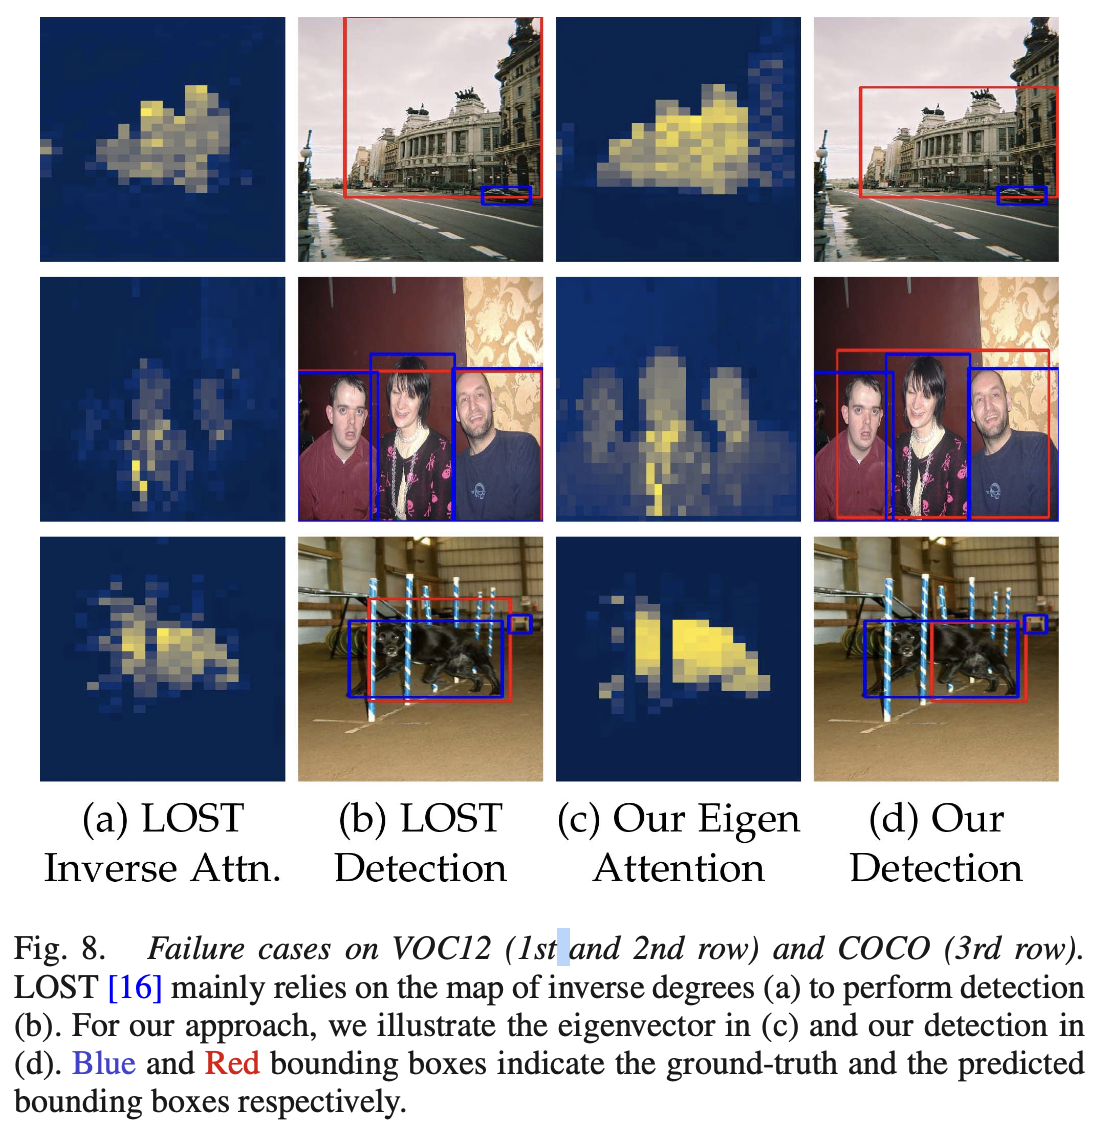
\includegraphics[width=0.7\linewidth]{Proposal_image.png}
\end{figure}
\end{frame}

% ---------- FRAME 4 ----------
\begin{frame}{Motivation}
\begin{itemize}
    \item TokenCut performs well in clean, single-object scenarios but the above failure modes limit its applicability in real-world images.
    \item \textbf{Goal:} Targeted extensions that address these limitations while preserving the core NCut pipeline.
    \item \textbf{Two directions explored:}
    \begin{enumerate}
        \item \textbf{Occlusion handling} — Graph Diffusion, Spatial Affinity Term
        \item \textbf{Multi-object detection} — Recursive detection and combined variants
    \end{enumerate}
    \item \textbf{Code:} Core TokenCut pipeline from the official GitHub repository; all extensions and modifications coded from scratch.
\end{itemize}
\end{frame}

% ---------- METHOD 1: Graph Diffusion ----------
\begin{frame}{Method 1: Graph Diffusion}
\begin{itemize}
    \item \textbf{Idea:} Two-hop connections in the graph bridge object parts separated by occluder patches.
    \item \textbf{Modified affinity:}
    \[
        E' = E + \gamma E^2, \quad E^2_{ij} = \textstyle\sum_k E_{ik}\,E_{kj}
    \]
    \item Indirect similarity through intermediate patch $k$ compensates for broken direct edges.
    \item Hyper-parameter $\gamma$ controls the diffusion strength.
\end{itemize}
\end{frame}

\begin{frame}{Method 1: Graph Diffusion — Results}
\centering
\small\textbf{Extension performs better}\\[0.15em]

\includegraphics[width=0.45\linewidth,height=0.33\textheight,keepaspectratio]{comparison_avg_diffusion/modified_wins/001_000017.jpg}\hfill
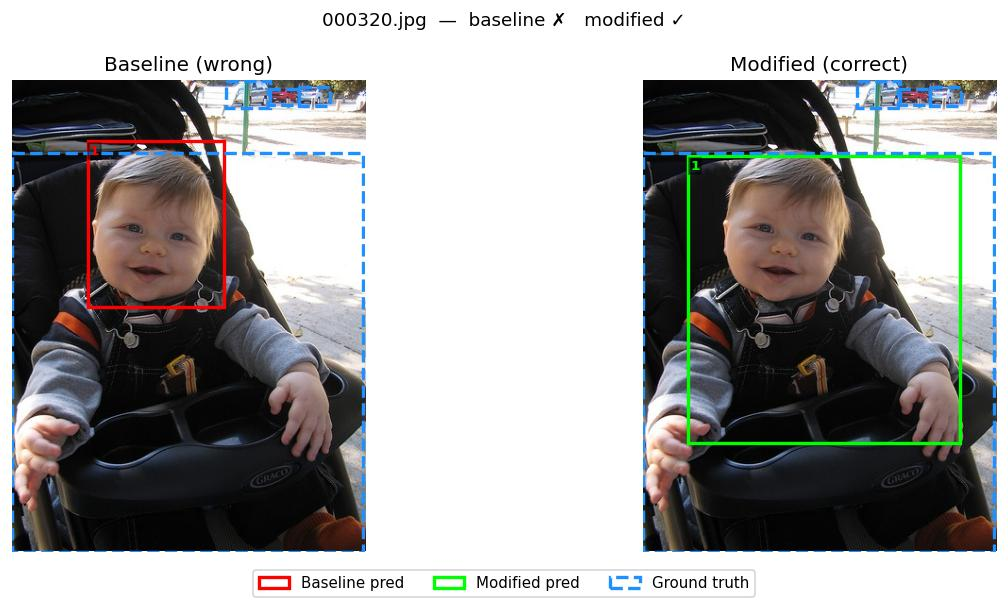
\includegraphics[width=0.45\linewidth,height=0.33\textheight,keepaspectratio]{comparison_avg_diffusion/modified_wins/011_000320.jpg}\\[0.3em]
\small\textbf{Base performs better}\\[0.15em]
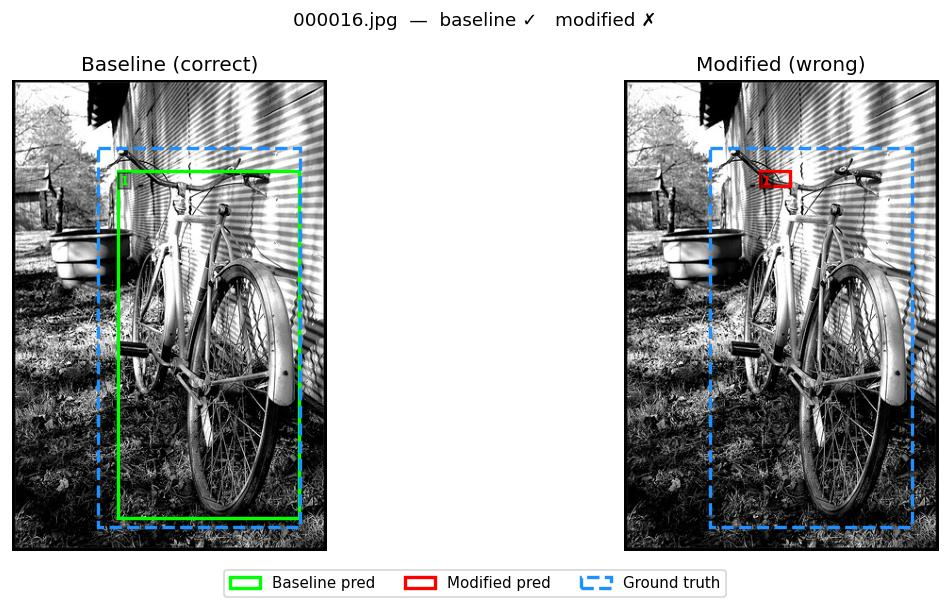
\includegraphics[width=0.45\linewidth,height=0.33\textheight,keepaspectratio]{comparison_avg_diffusion/baseline_wins/001_000016.jpg}\hfill
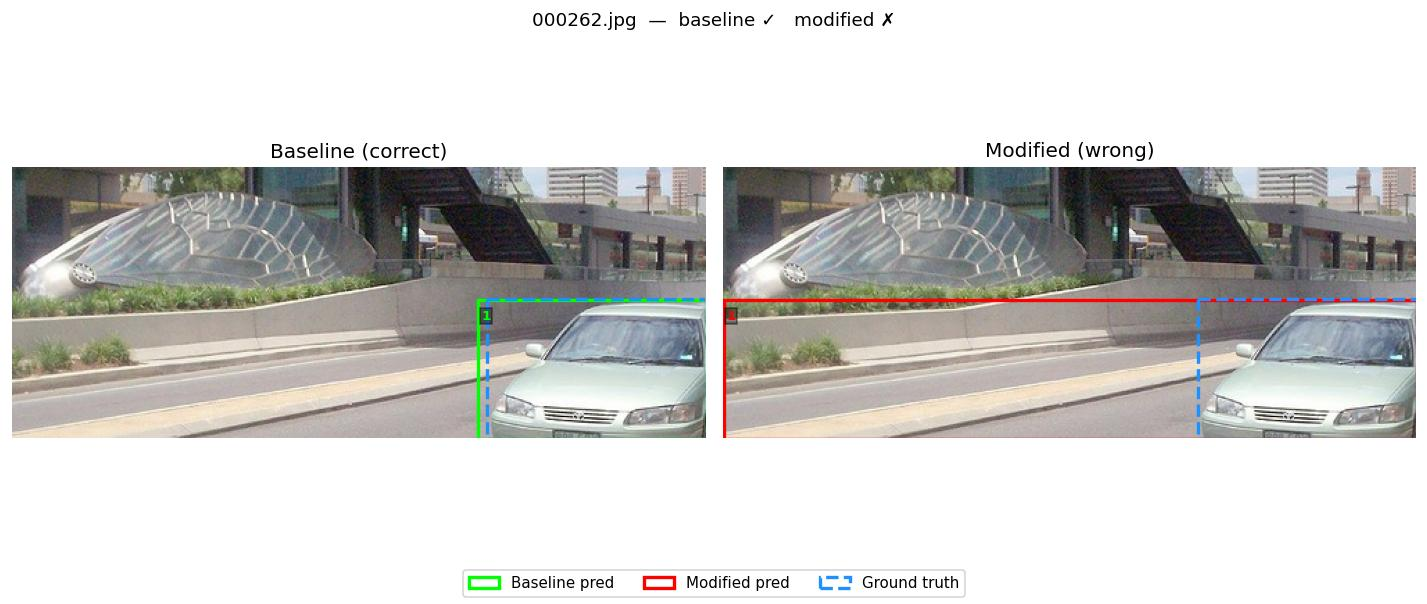
\includegraphics[width=0.45\linewidth,height=0.33\textheight,keepaspectratio]{comparison_avg_diffusion/baseline_wins/005_000262.jpg}
\end{frame}

% ---------- METHOD 2: Spatial Affinity ----------
\begin{frame}{Method 2: Spatial Affinity Term}
\begin{itemize}
    \item \textbf{Idea:} Spatially adjacent patches should stay connected regardless of appearance changes.
    \item \textbf{Spatial term:}
    \[
        S_{ij} = \exp\!\left(-\frac{\|p_i - p_j\|^2}{2\sigma^2}\right)
    \]
    \item \textbf{Combined affinity:} $A_{ij} = (1-\alpha)\,W_{ij} + \alpha\,S_{ij}$
    \item Spatial smoothness prevents over-fragmentation of the affinity graph under local occlusion.
\end{itemize}
\end{frame}

\begin{frame}{Method 2: Spatial Affinity Term — Results}
\centering
\small\textbf{Extension performs better}\\[0.15em]

\includegraphics[width=0.45\linewidth,height=0.33\textheight,keepaspectratio]{comparison_avg_spatial/modified_wins/001_000017.jpg}\hfill

\includegraphics[width=0.45\linewidth,height=0.33\textheight,keepaspectratio]{comparison_avg_spatial/modified_wins/023_002609.jpg}\\[0.3em]
\small\textbf{Base performs better}\\[0.15em]

\includegraphics[width=0.45\linewidth,height=0.33\textheight,keepaspectratio]{comparison_avg_spatial/baseline_wins/004_000211.jpg}\hfill

\includegraphics[width=0.45\linewidth,height=0.33\textheight,keepaspectratio]{comparison_avg_spatial/baseline_wins/005_000222.jpg}
\end{frame}

% ---------- QUALITATIVE COMPARISON ----------
\begin{frame}{Qualitative Comparison — Occlusion Methods}
\centering
\begin{minipage}{0.22\linewidth}
    \centering
    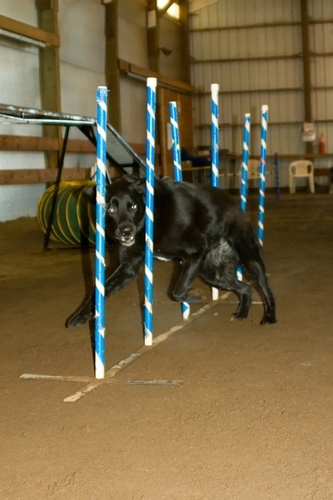
\includegraphics[width=\linewidth,height=0.6\textheight,keepaspectratio]{000112.jpg}\\[0.3em]
    \scriptsize\textbf{Original}
\end{minipage}\hfill
\begin{minipage}{0.22\linewidth}
    \centering
    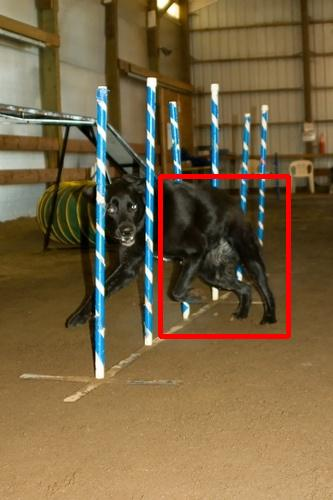
\includegraphics[width=\linewidth,height=0.6\textheight,keepaspectratio]{000112_TokenCut_pred_baseline.jpg}\\[0.3em]
    \scriptsize\textbf{Baseline}
\end{minipage}\hfill
\begin{minipage}{0.22\linewidth}
    \centering
    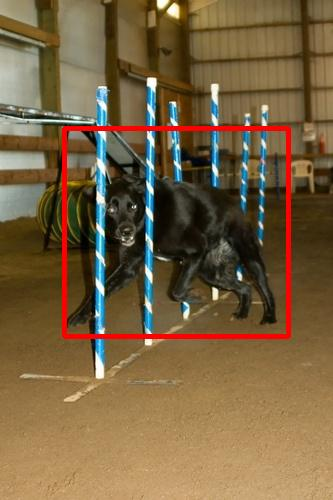
\includegraphics[width=\linewidth,height=0.6\textheight,keepaspectratio]{000112_TokenCut_pred_diffusion_02.jpg}\\[0.3em]
    \scriptsize\textbf{Graph Diffusion}
\end{minipage}\hfill
\begin{minipage}{0.22\linewidth}
    \centering
    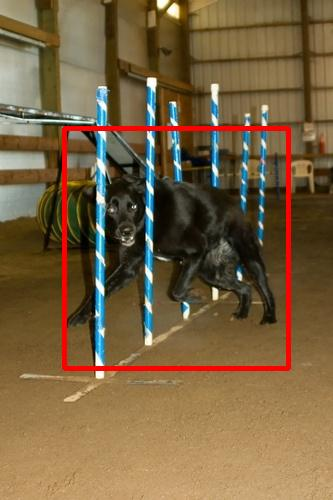
\includegraphics[width=\linewidth,height=0.6\textheight,keepaspectratio]{000112_TokenCut_pred_spatial.jpg}\\[0.3em]
    \scriptsize\textbf{Spatial Affinity}
\end{minipage}
\end{frame}

% ---------- METHOD 3: Recursive ----------
\begin{frame}{Method 3: Recursive Detection}
\begin{itemize}
    \item \textbf{Idea:} Detect one object per iteration; mask it out and re-run TokenCut on the residual graph.
    \item \textbf{Algorithm:}
    \begin{enumerate}
        \item Run TokenCut $\rightarrow$ foreground mask $M_k$.
        \item Remove $M_k$ patches from graph; re-run NCut on remaining nodes.
        \item Terminate when $\lambda_2 > \lambda_{\text{stop}}$ (no clear partition remains).
    \end{enumerate}
    \item Sequentially discovers multiple objects without altering the core bipartition.
\end{itemize}
\end{frame}

\begin{frame}{Method 3: Recursive Detection — Results}
\centering
\small\textbf{Extension performs better}\\[0.15em]
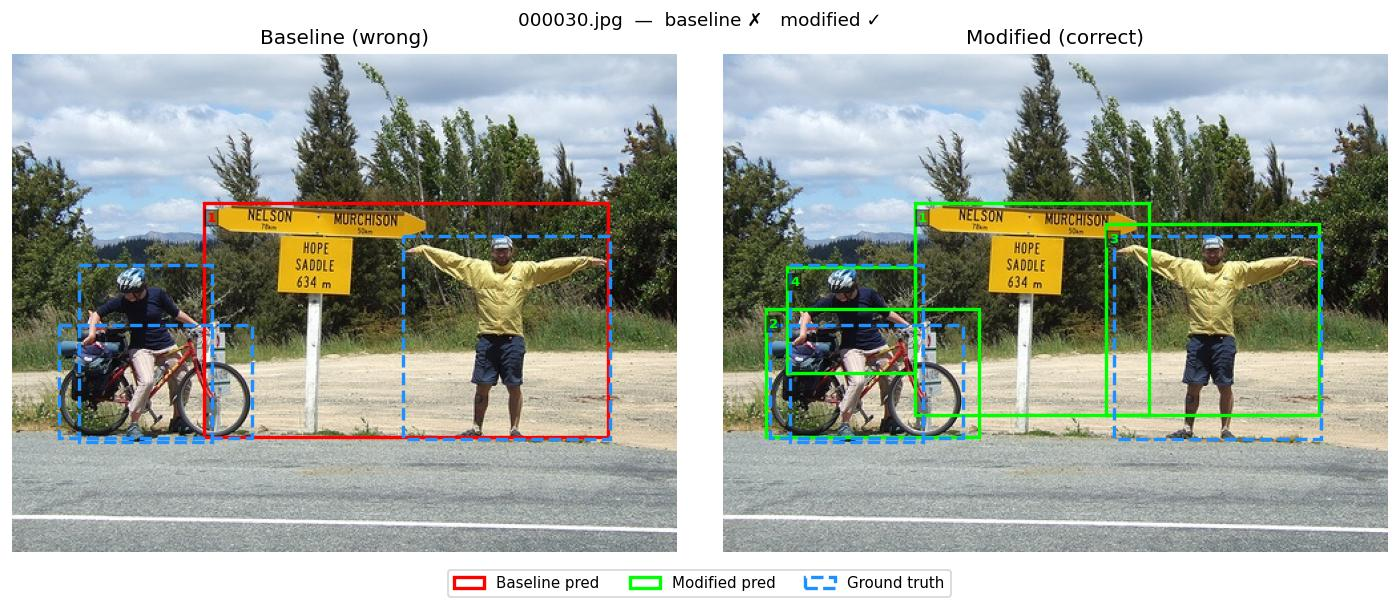
\includegraphics[width=0.45\linewidth,height=0.33\textheight,keepaspectratio]{comparison_avg_recursive_minbox/modified_wins/001_000030.jpg}\hfill
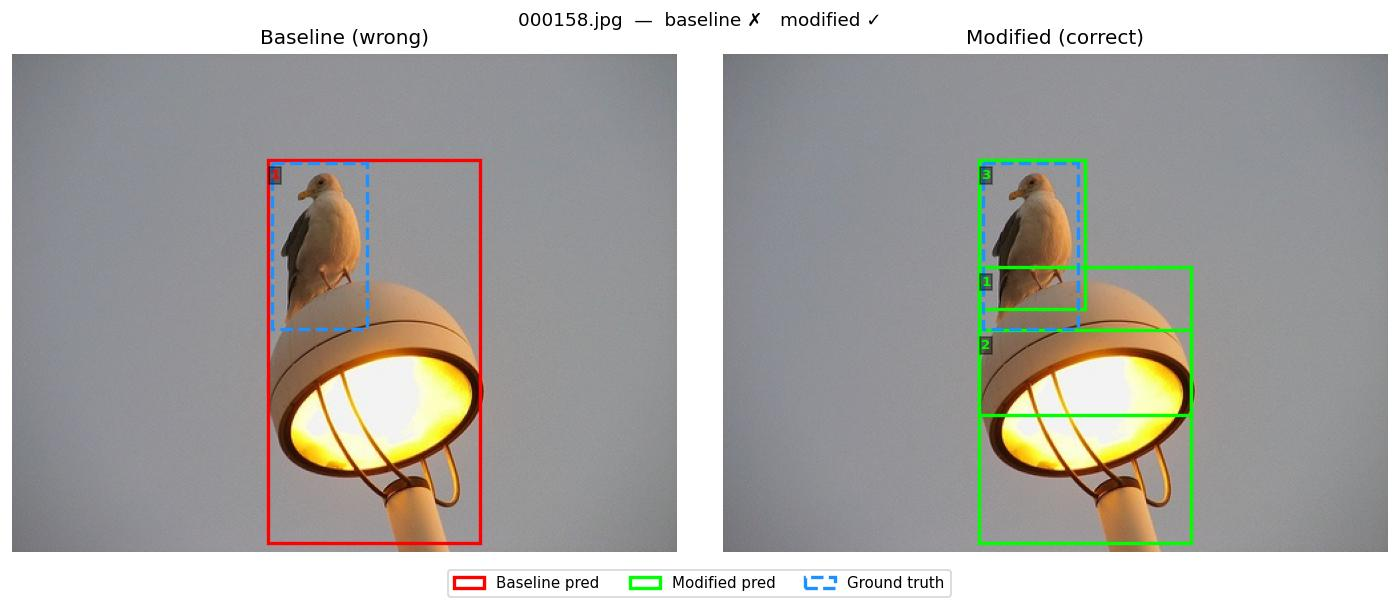
\includegraphics[width=0.45\linewidth,height=0.33\textheight,keepaspectratio]{comparison_avg_recursive_minbox/modified_wins/005_000158.jpg}\\[0.3em]
\small\textbf{Base performs better}\\[0.15em]
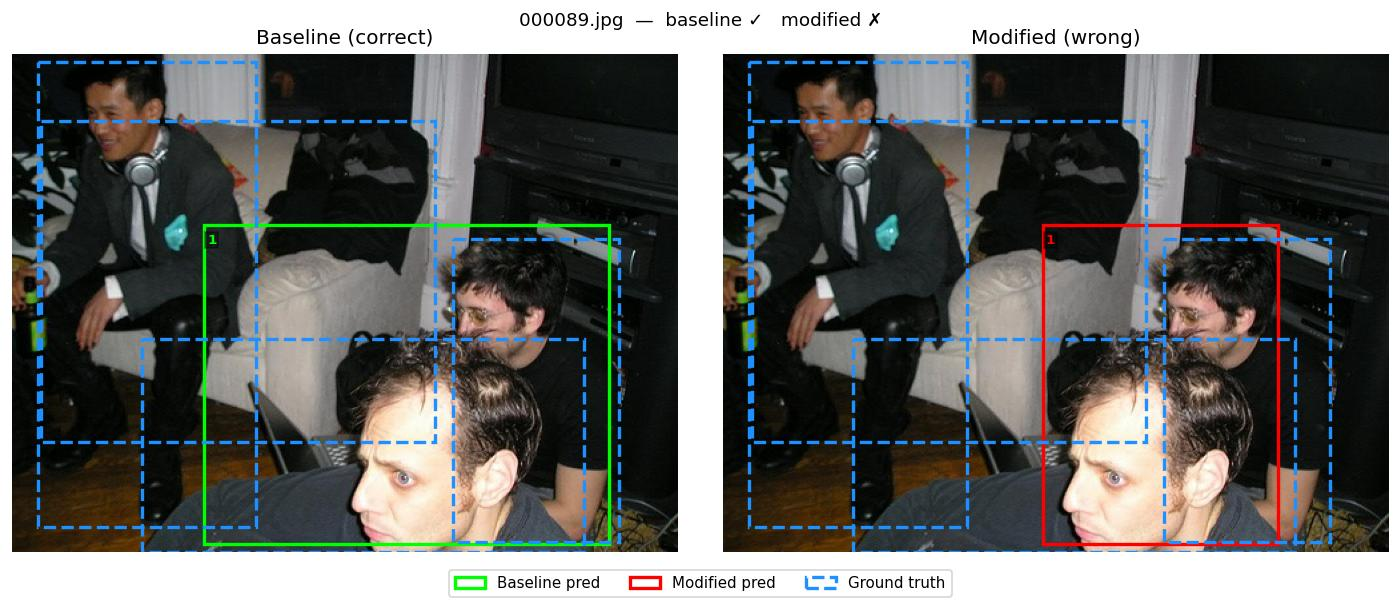
\includegraphics[width=0.45\linewidth,height=0.33\textheight,keepaspectratio]{comparison_avg_recursive_minbox/baseline_wins/001_000089.jpg}\hfill
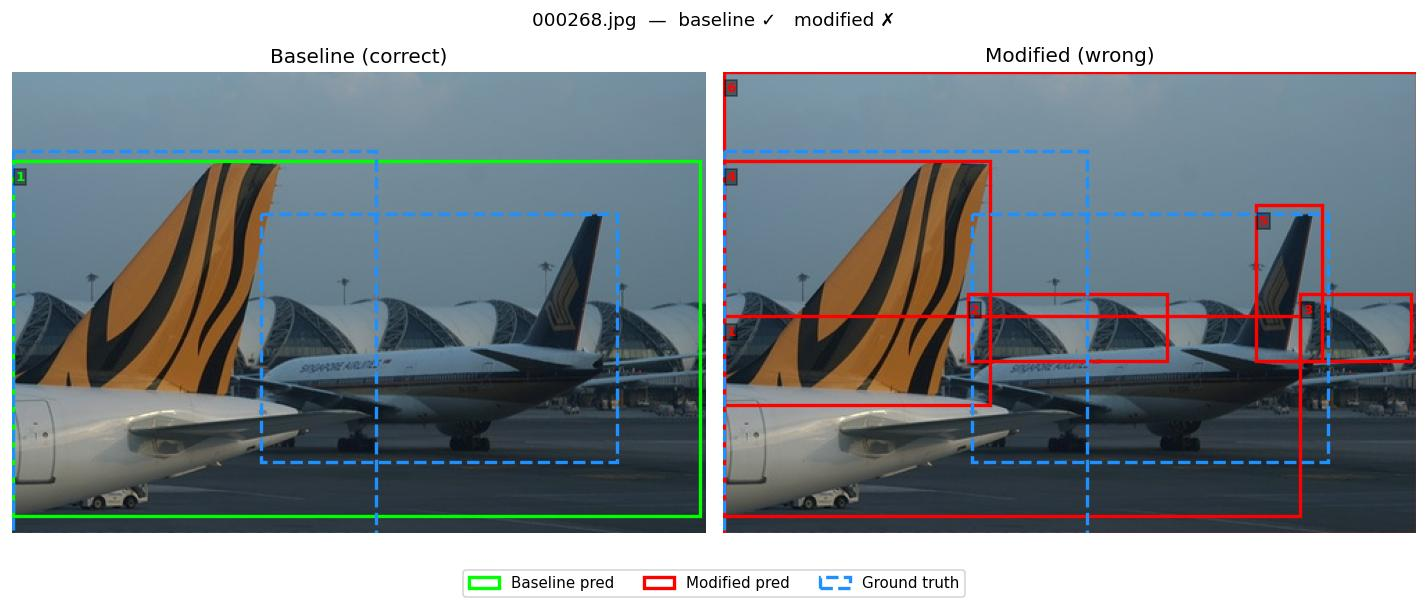
\includegraphics[width=0.45\linewidth,height=0.33\textheight,keepaspectratio]{comparison_avg_recursive_minbox/baseline_wins/005_000268.jpg}
\end{frame}

% ---------- METHOD 4: Recursive + Spatial ----------
\begin{frame}{Method 4: Recursive + Spatial Affinity — Results}
\centering
\small\textbf{Extension performs better}\\[0.15em]
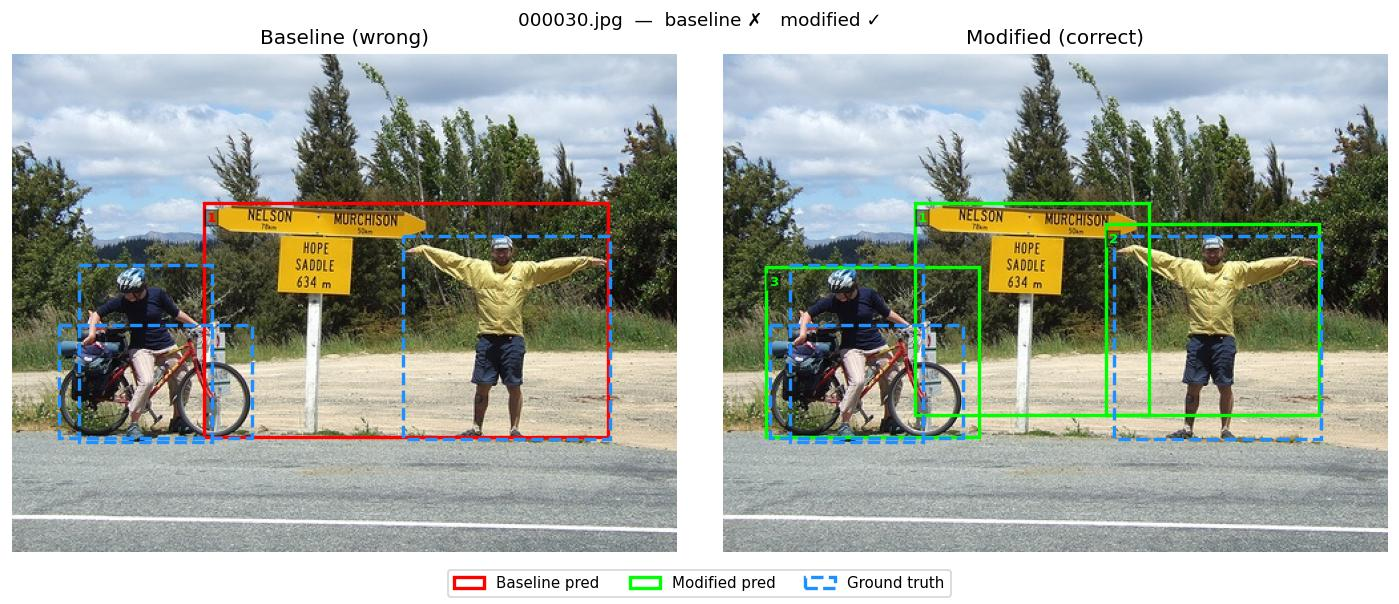
\includegraphics[width=0.45\linewidth,height=0.33\textheight,keepaspectratio]{comparison_avg_recursive_spatial_minbox/modified_wins/001_000030.jpg}\hfill
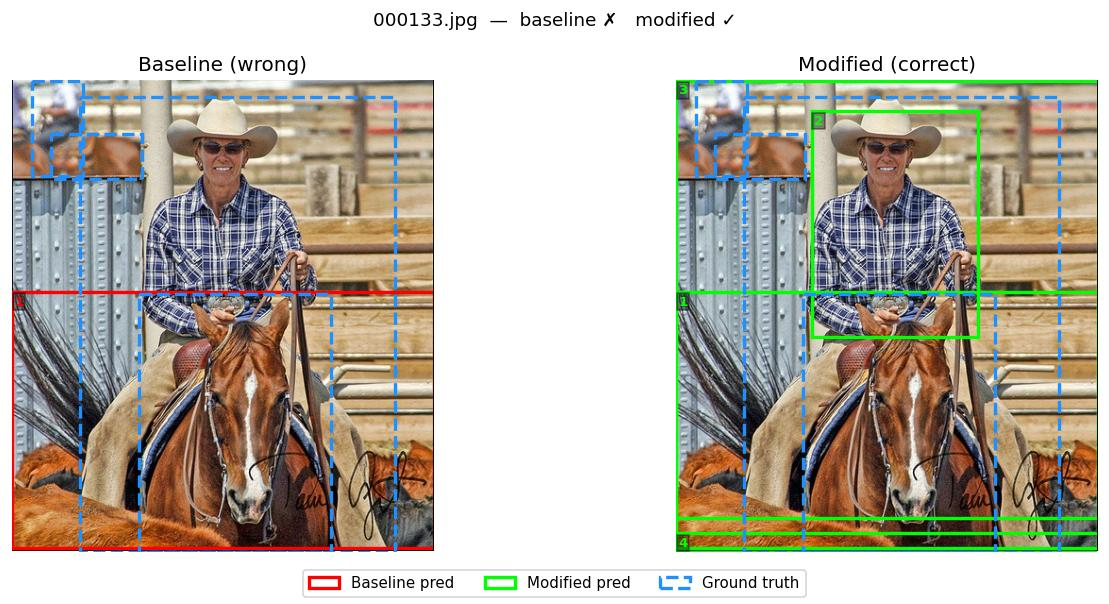
\includegraphics[width=0.45\linewidth,height=0.33\textheight,keepaspectratio]{comparison_avg_recursive_spatial_minbox/modified_wins/005_000133.jpg}\\[0.3em]
\small\textbf{Base performs better}\\[0.15em]
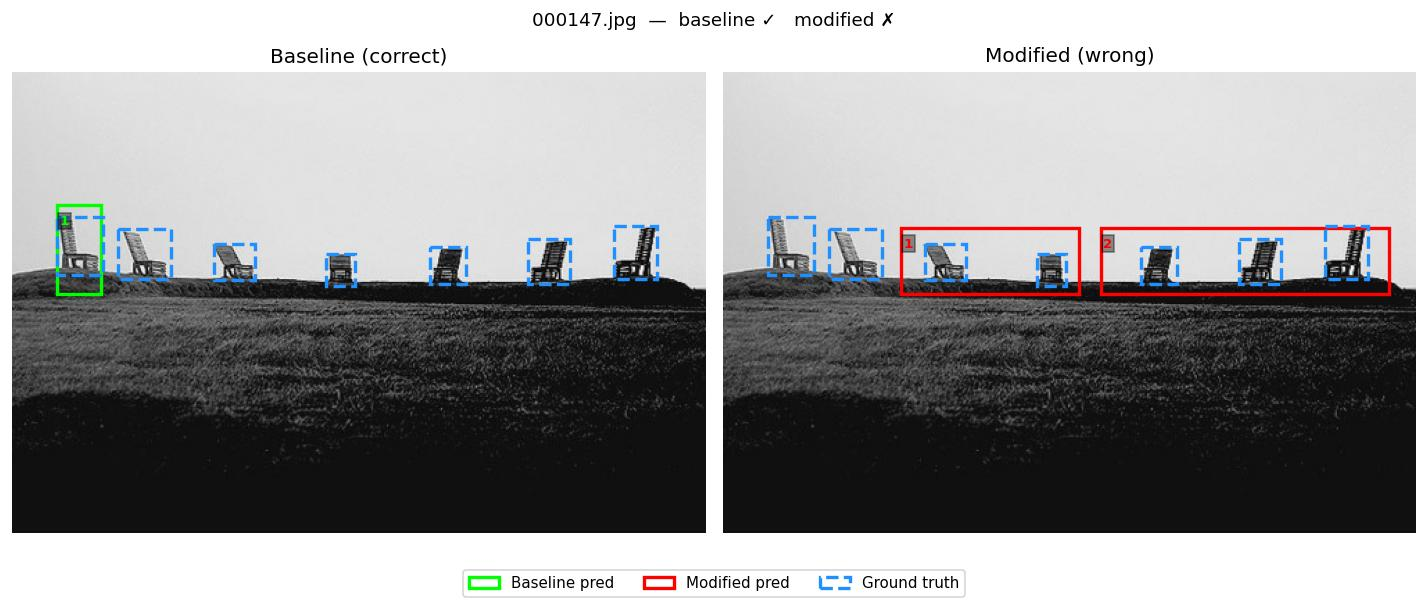
\includegraphics[width=0.45\linewidth,height=0.33\textheight,keepaspectratio]{comparison_avg_recursive_spatial_minbox/baseline_wins/001_000147.jpg}\hfill
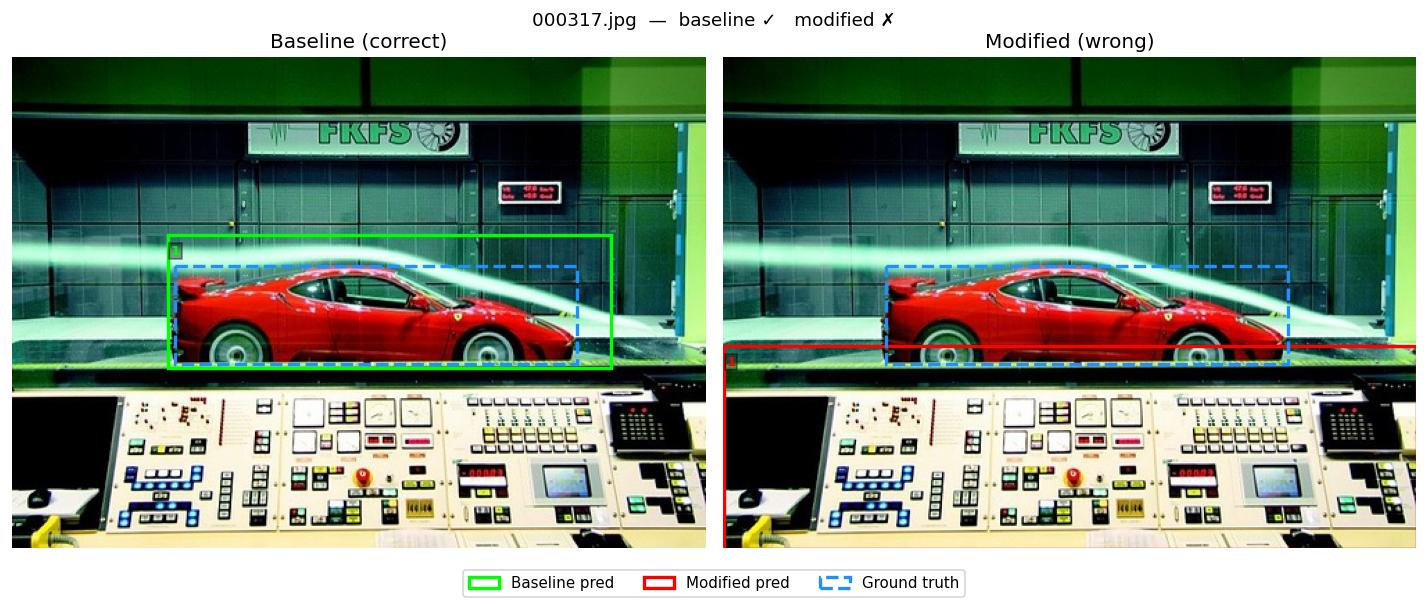
\includegraphics[width=0.45\linewidth,height=0.33\textheight,keepaspectratio]{comparison_avg_recursive_spatial_minbox/baseline_wins/005_000317.jpg}
\end{frame}

% ---------- METHOD 5: Spatial + Recursive + Min Box Area ----------

\begin{frame}{Method 5: Recursive + Diffusion — Results}
\centering
\small\textbf{Extension performs better}\\[0.15em]
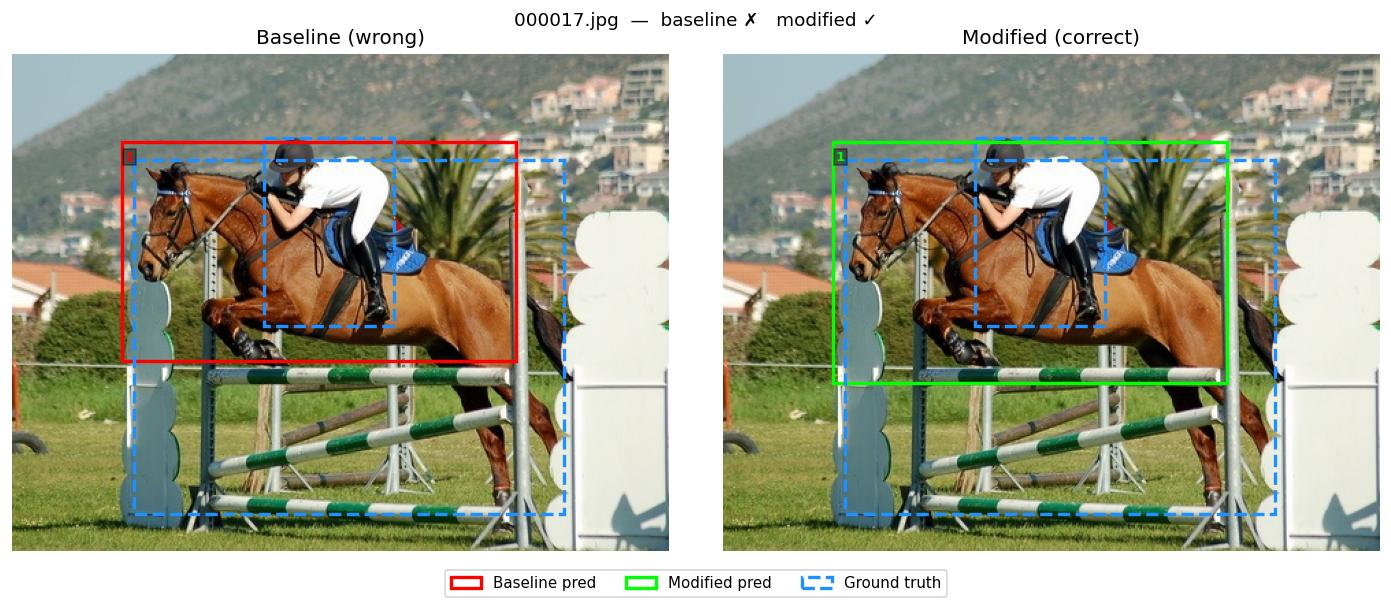
\includegraphics[width=0.45\linewidth,height=0.33\textheight,keepaspectratio]{comparison_avg_recursive_diffusion_minbox/modified_wins/001_000017.jpg}\hfill
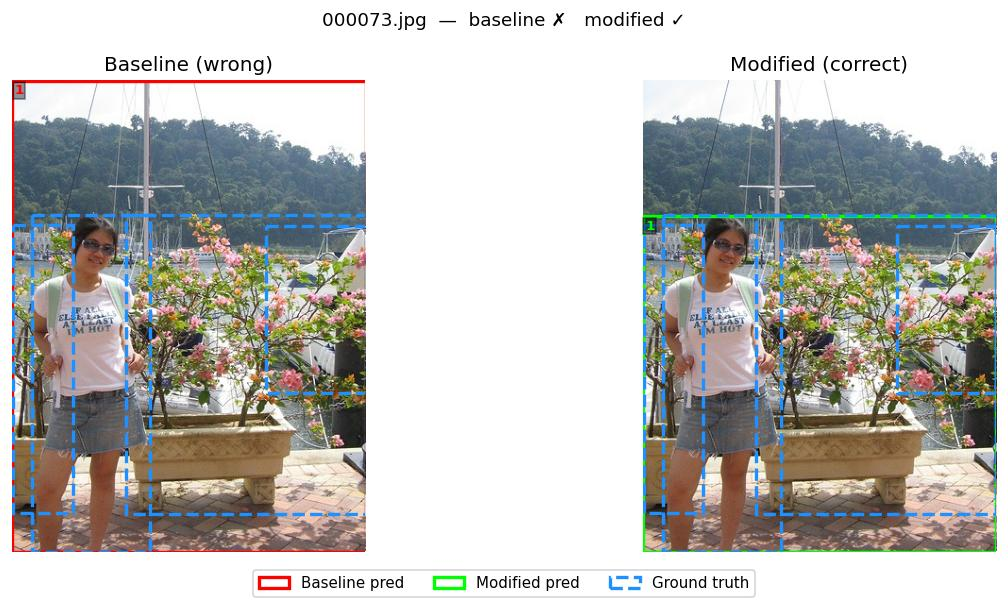
\includegraphics[width=0.45\linewidth,height=0.33\textheight,keepaspectratio]{comparison_avg_recursive_diffusion_minbox/modified_wins/005_000073.jpg}\\[0.3em]
\small\textbf{Base performs better}\\[0.15em]
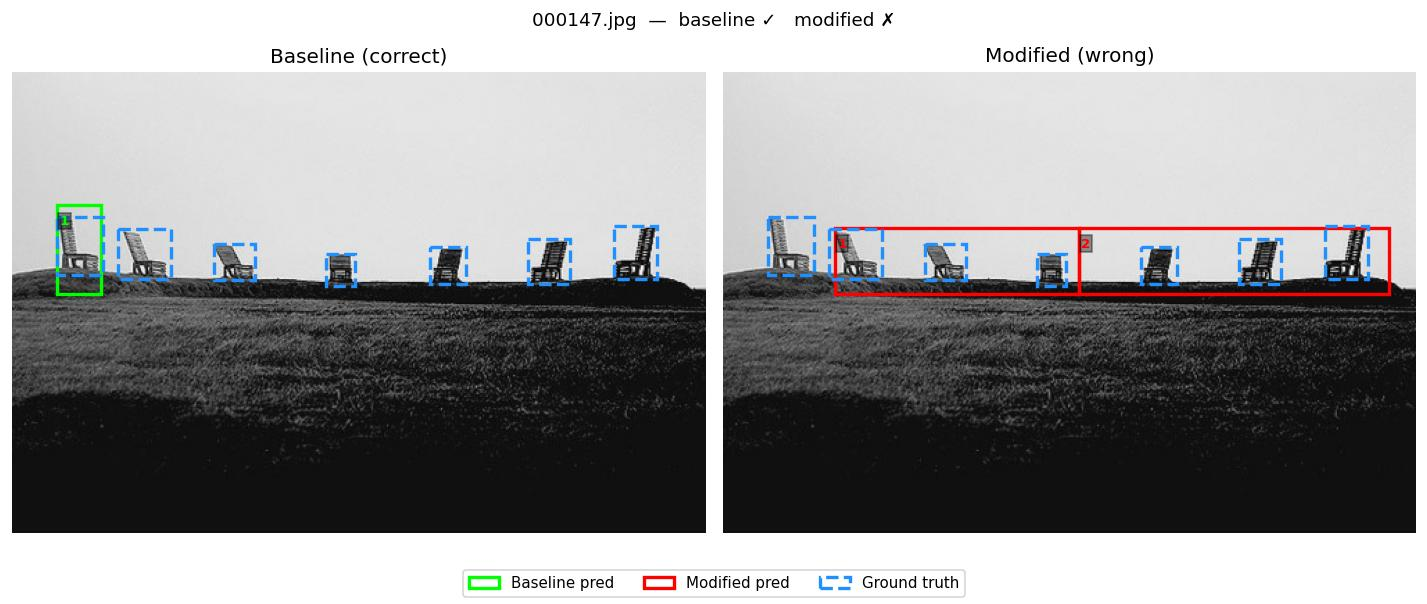
\includegraphics[width=0.45\linewidth,height=0.33\textheight,keepaspectratio]{comparison_avg_recursive_diffusion_minbox/baseline_wins/001_000147.jpg}\hfill
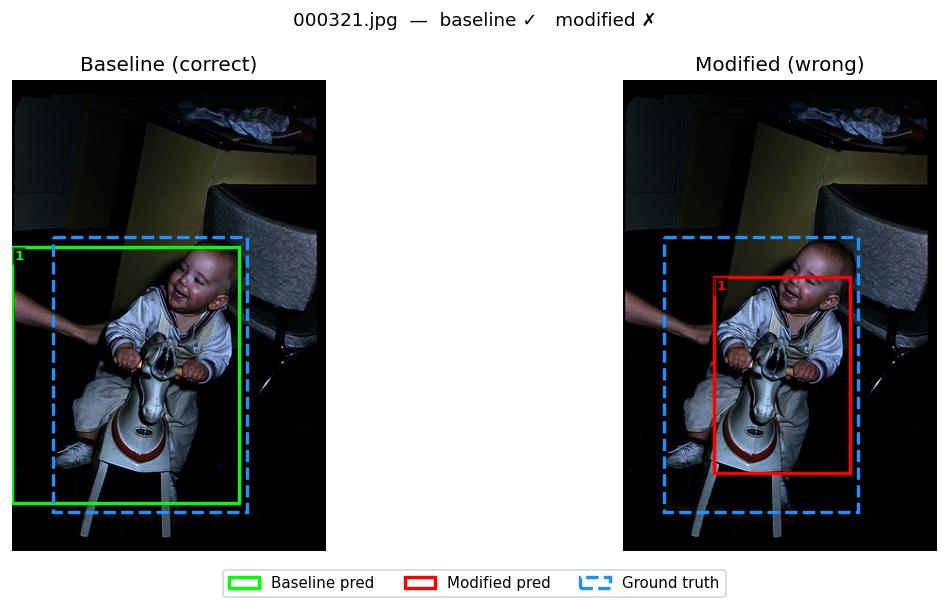
\includegraphics[width=0.45\linewidth,height=0.33\textheight,keepaspectratio]{comparison_avg_recursive_diffusion_minbox/baseline_wins/005_000321.jpg}
\end{frame}

% ---------- QUANTITATIVE RESULTS ----------
\begin{frame}{Quantitative Results}
\vspace{0.1cm}
\resizebox{\textwidth}{!}{%
\renewcommand{\arraystretch}{1.6}
\begin{tabular}{l|c|c|c|c|c|c}
\toprule
\textbf{Dataset} & \textbf{Baseline} & \textbf{Diffusion} & \textbf{Spatial} & \textbf{Recursive} & \textbf{Rec.+Spatial} & \textbf{Rec.+Diffusion} \\
\midrule
VOC07 & 68.71 & 66.71 & 66.79 & \textbf{72.90} & 70.50 & 68.77 \\
VOC12 & 72.07 & 69.27 & 71.12 & \textbf{75.51} & 75.23 & 71.41 \\
\bottomrule
\end{tabular}%
}
\vspace{0.2cm}\\
\tiny Metric: CorLoc (\%). Unsupervised single object discovery on VOC07 and VOC12. \textbf{Bold} = best.
\end{frame}

% ---------- END SLIDE ----------
\begin{frame}{}
    \centering
    \Huge{Thank You!}
    \vspace{1cm}
\end{frame}

\end{document}
